\subsection{Dated Pilot Mechanism Audit}
After the pilot and the original held-out freeze, the revised question asks when
repetition protects information from summary loss and when it obscures meaningful
differences. The dated amendment preserves H1--H4 and their original analyses;
new mechanism analyses of those runs are exploratory. No original held-out model
choices were inspected to design the amendment. Its new confirmatory contrasts
require disjoint, prospectively frozen instances.

The pilot comprises 24 independent base pairs, not 1,152 independent observations.
All repeated reports are correct. No selected objective favors a fastest infeasible
candidate. Mandatory Boolean retention is near ceiling; numerical objectives
sometimes become Boolean values or disappear despite syntactically valid JSON.
Other errors occur after the correct failed constraint reaches the root. Therefore
the pilot does not identify a single retention mechanism.
\begin{figure}[ht]
\centering
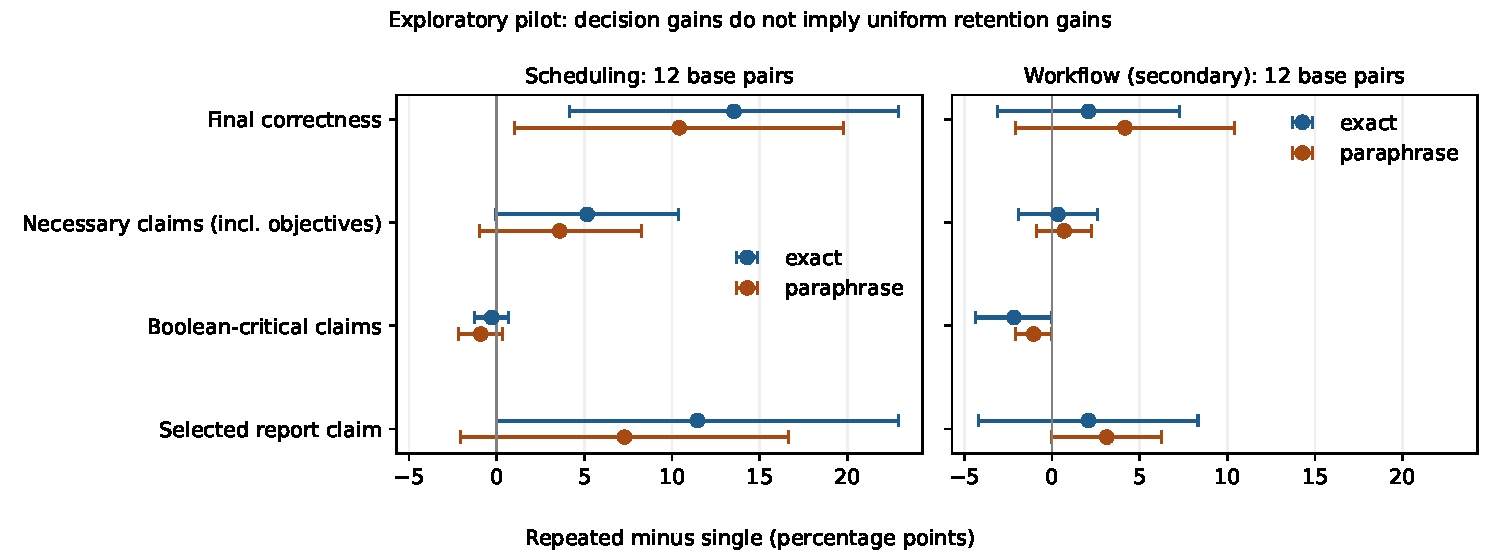
\includegraphics[width=\textwidth]{../results/pilot-mechanism-v1/figures/retention-and-decisions.pdf}
\caption{Exploratory pilot: paired changes in correctness and explicit retention.
Intervals resample independent base pairs, stratified by mutation family and
change status. Necessary scopes include numerical objectives; Boolean-critical
scopes use a truth-value-flip definition. These metrics do not observe hidden reasoning.}
\label{fig:mechanism-pilot}
\end{figure}

Unexposed-manager prompts and requested seeds matched in 192 paired comparisons
per population. Normalized findings nevertheless differed in two workflow
comparisons and none in scheduling. New tests share identical manager computations
within a world and stochastic repetition, including the bypass control. This is
a new coupling intervention, not a retrospective repair of pilot outputs.
